This system contains the video input subsystem, the video output subsystem, and the gimbal controller subsystem. Each subsystem makes it possible for this system to communicate with the Camera System Layer and the Virtual Reality System Layer. Video data will be received from the Camera System Layer and transferred to the Virtual Reality System Layer, while angular data will be received from the Virtual Reality System Layer and sent to the Camera System Layer.

\begin{figure}[h!]
	\centering
 	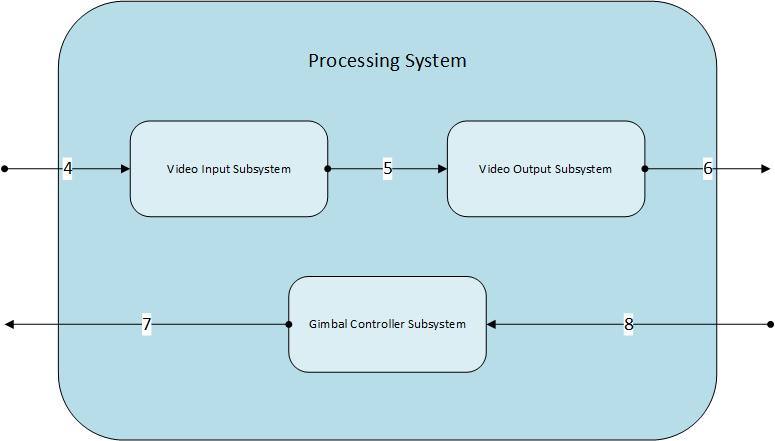
\includegraphics[width=0.75\textwidth]{images/processingsubsystem}
 \caption{Microcomputer System Layer Subsystem Description Diagram}
\end{figure}

\subsection{Video Input Subsystem}
This subsystem communicates with the camera subsystem in the Camera System Layer. Also, the video interface subsystem interacts with the video output subsystem in this system.

\subsubsection{Assumptions}
None

\subsubsection{Responsibilities}
This subsystem will receive raw video data sent from the Camera System Layer. The raw video data will then be processed and sent to the video output subsystem in this system.

\subsubsection{Subsystem Interfaces}

\begin {table}[H]
\caption {Video Input Subsystem interfaces} 
\begin{center}
    \begin{tabular}{ | p{1cm} | p{6cm} | p{3cm} | p{3cm} |}
    \hline
    ID & Description & Inputs & Outputs \\ \hline
    \#5 & Camera System - Camera Subsystem & \pbox{3cm}{Raw video data} & \pbox{3cm}{N/A}  \\ \hline
    \#6 & Video Output Subsystem & \pbox{3cm}{N/A} & \pbox{3cm}{Processed video data}  \\ \hline
    \end{tabular}
\end{center}
\end{table}

\subsection{Video Output Subsystem}
This subsystem interacts with the video input subsystem in this system, and it will be one of the means of communication between the Processing System Layer and the Virtual Reality System Layer.

\subsubsection{Assumptions}
None

\subsubsection{Responsibilities}
Processed video data is received from the video input subsystem in this system. With the video data, it will be transferred to the Virtual Reality System Layer to be displayed.

\subsubsection{Subsystem Interfaces}

\begin {table}[H]
\caption {Video Output Subsystem interfaces} 
\begin{center}
    \begin{tabular}{ | p{1cm} | p{6cm} | p{3cm} | p{3cm} |}
    \hline
    ID & Description & Inputs & Outputs \\ \hline
    \#7 & Video Input Subsystem & \pbox{3cm}{Processed video data} & \pbox{3cm}{N/A}  \\ \hline
    \#8 & Virtual Reality System - Stereo Display Subsystem & \pbox{3cm}{N/A} & \pbox{3cm}{Processed video data}  \\ \hline
    \end{tabular}
\end{center}
\end{table}

\subsection{Gimbal Controller Subsystem}
This subsystem interacts with the gimbal controller subsystem of the Camera System Layer and the head tracking subsystem of the Virtual Reality System Layer.

\subsubsection{Assumptions}
None

\subsubsection{Responsibilities}
This subsystem will take the raw angular data taken from the virtual reality headset of the Virtual Reality System Layer and send it to the gimbal controller subsystem of the Camera System Layer through serial communication.

\subsubsection{Subsystem Interfaces}

\begin {table}[H]
\caption {Gimbal Controller Subsystem interfaces} 
\begin{center}
    \begin{tabular}{ | p{1cm} | p{6cm} | p{3cm} | p{3cm} |}
    \hline
    ID & Description & Inputs & Outputs \\ \hline
    \#9 & Camera System - Gimbal Controller Subsystem & \pbox{3cm}{N/A} & \pbox{3cm}{Head tracking angles}  \\ \hline
    \#10 & Virtual Reality System - Stereo Display Subsystem & \pbox{3cm}{Raw head tracking angles} & \pbox{3cm}{N/A}  \\ \hline
    \end{tabular}
\end{center}
\end{table}